% 难度：★★★ 难题
% 知识点：立体几何，折叠问题，动点轨迹，坐标系

\newcommand{\qSolidTrapFoldArcStem}{
等腰梯形 $ABCD$ 中，$AB\parallel CD$，$AB=2$，$AD=BC=1$，$AB>CD$．沿着 $AC$ 把 $\triangle ACD$ 折起至 $\triangle ACD_1$，使 $D_1$ 在平面 $ABC$ 上的射影恰好落在 $AB$ 上．当边长 $CD$ 变化时，求点 $D_1$ 的轨迹长度．
}

\newcommand{\qSolidTrapFoldArcOptions}{
A. $\frac{\pi}{2}$ \hfill
B. $\frac{\pi}{3}$ \hfill
C. $\frac{\pi}{4}$ \hfill
D. $\frac{\pi}{6}$
}

\newcommand{\qSolidTrapFoldArcFigure}{
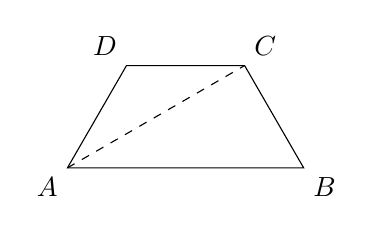
\begin{tikzpicture}[scale=1.5]
  \coordinate (A) at (0,0);
  \coordinate (B) at (2,0);
  \coordinate (C) at (1.5, 0.866);
  \coordinate (D) at (0.5, 0.866);
  
  \draw (A) -- (B) -- (C) -- (D) -- cycle;
  \draw[dashed] (A) -- (C);
  
  \node[below left] at (A) {$A$};
  \node[below right] at (B) {$B$};
  \node[above right] at (C) {$C$};
  \node[above left] at (D) {$D$};
\end{tikzpicture}
}

\newcommand{\qSolidTrapFoldArcAnswer}{
B
}

\newcommand{\qSolidTrapFoldArcSolution}{
\textbf{【分析】}

设 $D_1$ 在平面 $ABC$ 上的射影为 $H$，则 $H \in AB$．
因为 $D_1H \perp$ 平面 $ABC$，且 $AB \subset$ 平面 $ABC$，所以 $D_1H \perp AB$．
这就意味着点 $D_1$ 始终位于过直线 $AB$ 且垂直于平面 $ABC$ 的平面（即竖直平面）内．
又因为折叠过程中线段 $AD_1$ 的长度保持不变，即 $AD_1 = AD = 1$．
所以在该竖直平面内，点 $D_1$ 到定点 $A$ 的距离恒为 $1$，点 $D_1$ 的轨迹是半径为 $1$ 的圆的一段弧．
我们只需要求出 $H$ 在 $AB$ 上运动的范围，即可确定圆心角的范围，从而求出弧长．

\textbf{【求解】}

在折叠前的等腰梯形 $ABCD$ 中，设 $\angle DAB = \theta$．
因为 $AD=BC=1$，$AB=2$，所以 $A$ 到 $D$ 在 $AB$ 上投影的距离为 $\cos\theta$，
$CD = 2 - 2\cos\theta$．由 $0 < CD < AB$ 可得 $0 < 2 - 2\cos\theta < 2$，即 $\cos\theta \in (0, 1)$．
以 $A$ 为原点，$AB$ 所在直线为 $x$ 轴建立平面直角坐标系，
则 $A(0,0)$，$C(2-\cos\theta, \sin\theta)$，$D(\cos\theta, \sin\theta)$．
向量 $\overrightarrow{AC} = (2-\cos\theta, \sin\theta)$．

设折叠后 $D_1$ 的射影 $H$ 的坐标为 $(x, 0)$，其中 $x$ 即为线段 $AH$ 的长度．
设 $P$ 为 $D_1$ 在 $AC$ 上的射影，则 $P$ 也是 $D$ 在 $AC$ 上的射影（折叠不改变面内投影点）．
由三垂线定理逆定理，因为 $D_1H \perp$ 平面 $ABC$，$D_1P \perp AC$，所以 $HP \perp AC$．
这表明在折叠前的平面图形中，直线 $DH$ 垂直于 $AC$．
所以 $\overrightarrow{DH} \cdot \overrightarrow{AC} = 0$．
$\overrightarrow{DH} = (x-\cos\theta, -\sin\theta)$，代入得：
$$(x-\cos\theta)(2-\cos\theta) - \sin^2\theta = 0$$
整理得：$x(2-\cos\theta) = 2\cos\theta - \cos^2\theta + \sin^2\theta = 1 + 2\cos\theta - 2\cos^2\theta$．
令 $t = \cos\theta \in (0, 1)$，则 $x = \frac{-2t^2+2t+1}{2-t}$．

要使折叠在空间中能够实现，必须满足 $D_1H^2 \ge 0$．
在 $\text{Rt}\triangle D_1HP$ 中，$D_1H^2 = D_1P^2 - HP^2 = DP^2 - HP^2 \ge 0$，所以 $DP \ge HP$．
利用点到直线的距离公式求 $DP$ 和 $HP$（直线 $AC$ 方程为 $\sin\theta \cdot X - (2-\cos\theta) Y = 0$）：
$$DP = \frac{2(1-t)\sqrt{1-t^2}}{AC}, \quad HP = \frac{x\sqrt{1-t^2}}{AC}$$
由 $DP \ge HP$ 得 $2(1-t) \ge x$，即 $2-2t \ge \frac{-2t^2+2t+1}{2-t}$．
化简得 $4t^2 - 8t + 3 \ge 0$，即 $(2t-1)(2t-3) \ge 0$．
因为 $t \in (0, 1)$，所以 $t \le \frac{1}{2}$．
因此 $\cos\theta$ 的取值范围是 $(0, \frac{1}{2}]$．

考虑函数 $x(t) = \frac{-2t^2+2t+1}{2-t}$ 在 $(0, \frac{1}{2}]$ 上的单调性：
$x'(t) = \frac{2t^2 - 8t + 5}{(2-t)^2}$，由于方程 $2t^2 - 8t + 5 = 0$ 的小根为 $2 - \frac{\sqrt{6}}{2} > \frac{1}{2}$，
所以当 $t \in (0, \frac{1}{2}]$ 时，$x'(t) > 0$，函数单调递增．
当 $t \to 0$ 时，$x \to \frac{1}{2}$；当 $t = \frac{1}{2}$ 时，$x = 1$．
所以 $H$ 的横坐标 $x \in (\frac{1}{2}, 1]$．

在过 $AB$ 的竖直平面内，以 $A$ 为原点建立坐标系，点 $D_1$ 的坐标为 $(x, z)$，满足 $x^2 + z^2 = 1 (z>0)$．
设 $\angle D_1AH = \phi$，则 $\cos\phi = x$．
因为 $x \in (\frac{1}{2}, 1]$，所以 $\cos\phi \in (\frac{1}{2}, 1]$，从而 $\phi \in [0, \frac{\pi}{3})$．
点 $D_1$ 的轨迹是半径为 $1$、圆心角为 $\frac{\pi}{3}$ 的一段圆弧，其长度为 $\frac{\pi}{3}$．

故选 B．
}

\newcommand{\qSolidTrapFoldArcDiagnosis}{
\textbf{【学生常见问题】}
1. \textbf{未发现轨迹的共面性}：学生容易被“空间折叠”吓倒，没有通过条件“$D_1$ 射影在 $AB$ 上”敏锐地意识到点 $D_1$ 被锁死在过 $AB$ 的竖直平面内，而该平面内 $D_1A=1$ 意味着轨迹必为该平面内的一段圆弧．
2. \textbf{忽视折叠存在的几何限制}：本题最大的难点和易错点在于发现折叠的物理限制 $DP \ge HP$．如果不加判断，认为 $t=\cos\theta \in (0,1)$ 全程都能折叠，就会得出错误的 $x$ 范围，进而导致圆心角求错．
3. \textbf{平面坐标法基本功不扎实}：无法将“折叠不改变面内投影点”转化为平面图形中 $DH \perp AC$ 这一关键垂直关系．
}

\newcommand{\qSolidTrapFoldArcTeachingNotes}{
\textbf{【课堂处理建议】}
1. \textbf{提炼核心模型}：本题的第一个突破口是“空间动点的平面化”——“到定点的距离为定值”加“被限制在某个定平面内”（$D_1H \perp$ 平面 $ABC$ 且 $H \in AB$，说明 $D_1$ 始终在一个过 $AB$ 且垂直于底面的平面内），直接锁定轨迹是该平面内的圆弧．
2. \textbf{剖析“投影不变性”}：花 3-5 分钟带学生推导“面面折叠，折痕上的投影点不变”：无论折叠多少度，$D_1$ 在 $AC$ 上的投影永远是原来展开图中的 $P$ 点．借助三垂线定理理清 $D, H, P$ 在底面的位置关系，即 $DH \perp AC$．
3. \textbf{强调“存在性边界”}：一定要提问学生：“所有的梯形都能折出满足条件的 $D_1$ 吗？”借此引出空间直角三角形 $D_1HP$ 的勾股定理 $D_1H^2 = DP^2 - HP^2 \ge 0$ 这个隐藏的“存在性卡扣”．这一步是高端选拔题拉开差距的关键．
}
